% =====================================================================
%  GrapHist: Reproduction and a Proposed Correction  --  Group 1
%  Compile with: pdflatex graphist_presentation.tex   (run twice)
% =====================================================================
\documentclass[aspectratio=169,11pt]{beamer}

\usetheme{Boadilla}
\usepackage[T1]{fontenc}
\usepackage[utf8]{inputenc}
\usepackage{booktabs}
\usepackage{array}
\usepackage{tikz}
\usepackage{amsmath}
\usepackage{xcolor}
\usetikzlibrary{arrows.meta, positioning, shapes.geometric}

% ---------- colour identity: haematoxylin violet + eosin rose ----------
\definecolor{haem}{RGB}{74,56,145}
\definecolor{haemlight}{RGB}{237,233,248}
\definecolor{eosin}{RGB}{176,58,91}
\definecolor{eosinlight}{RGB}{250,237,241}
\definecolor{inkgrey}{RGB}{90,85,100}
\definecolor{goodgreen}{RGB}{46,107,79}

\setbeamercolor{structure}{fg=haem}
\setbeamercolor{title}{fg=white,bg=haem}
\setbeamercolor{frametitle}{fg=white,bg=haem}
\setbeamercolor{alerted text}{fg=eosin}
\setbeamercolor{block title}{fg=white,bg=haem}
\setbeamercolor{block body}{bg=haemlight}
\setbeamercolor{block title alerted}{fg=white,bg=eosin}
\setbeamercolor{block body alerted}{bg=eosinlight}
\setbeamertemplate{navigation symbols}{}
\setbeamertemplate{itemize items}[circle]
\setbeamerfont{frametitle}{size=\large}
\setbeamerfont{block title}{size=\small}

\newcommand{\um}{$\mu$m}
\newcommand{\hl}[1]{\textcolor{haem}{\textbf{#1}}}
\newcommand{\al}[1]{\textcolor{eosin}{\textbf{#1}}}


% =====================================================================
\title[GrapHist Reproduction]{GrapHist: Reproduction and a Proposed Correction}
\subtitle{Graph Self-Supervised Learning for Histopathology}
\author[Group 1: Aadith Krishna, Aditya Santosh, Arjungopal Anilkumar]{%
  \begin{tabular}{r@{\hspace{1.2em}}l}
    Aadith Krishna        & {\small CB.SC.U4AIE23202} \\[1pt]
    Aditya Santosh        & {\small CB.SC.U4AIE23207} \\[1pt]
    Arjungopal Anilkumar  & {\small CB.SC.U4AIE23271}
  \end{tabular}%
}
\institute{\textbf{Group 1}}
\date{}

\begin{document}

% ------------------------------------------------------------- 1
\begin{frame}[plain]
  \titlepage
\end{frame}

% ------------------------------------------------------------- 2
\begin{frame}{Introduction: why histopathology is hard for deep learning}

  A pathology slide is scanned into a \hl{Whole Slide Image (WSI)}, roughly
  $100{,}000 \times 80{,}000$ pixels and 1--3 GB per slide.

  \vspace{0.5em}
  \begin{columns}[T]
    \begin{column}{0.48\textwidth}
      \begin{block}{The standard approach}
        Cut the slide into small tiles, push each tile through a vision model
        such as a CNN or a Vision Transformer, then pool the tile features
        together.
      \end{block}
    \end{column}
    \begin{column}{0.48\textwidth}
      \begin{block}{Why it is unsatisfying}
        A vision transformer sees a \emph{fixed grid} of square patches. Real
        tissue is made of \emph{cells} at irregular positions. The grid does not
        line up with biology.
      \end{block}
    \end{column}
  \end{columns}

  \vspace{0.6em}
  \begin{alertblock}{The biological intuition}
    What matters diagnostically is \emph{which cells are present} and
    \emph{how they are arranged relative to each other}, not the raw pixels.
    That is naturally a \hl{graph}, not an image.
  \end{alertblock}

\end{frame}

% ------------------------------------------------------------- 3
\begin{frame}{Problem statement}

  \begin{alertblock}{The problem the paper sets out to solve}
    Vision models applied to histopathology are expensive to train, operate on a
    fixed grid that ignores cellular structure, and scale \emph{quadratically}
    with the number of image tokens.

    \vspace{0.4em}
    \textbf{Can tissue instead be represented as a graph of cells, so that a
    model learns cellular organisation directly, and does so at a much lower
    computational cost?}
  \end{alertblock}

  \vspace{0.6em}
  \begin{block}{Why this is a hard problem}
    \begin{itemize}\small
      \item Labels are scarce. Expert annotation of pathology slides is slow and
            expensive, so the model must learn \emph{without labels}.
      \item Tumour tissue is \emph{heterogeneous}. Neighbouring cells are often
            of different types, which breaks the assumption most graph networks
            are built on.
      \item A single slide can contain millions of cells, so the method has to
            stay cheap at scale.
    \end{itemize}
  \end{block}

\end{frame}

% ------------------------------------------------------------- 4
\begin{frame}{The base paper: what GrapHist is}

  \textbf{GrapHist: Graph Self-Supervised Learning for Histopathology}\\
  {\small Ö\u{g}üt et al., arXiv:2603.00143}

  \vspace{0.5em}
  \begin{block}{The thesis}
    Represent tissue as a \emph{cell graph}, pre-train on it without labels, and
    you obtain better representations than vision models at a fraction of the
    cost.
  \end{block}

  \vspace{0.3em}
  \begin{columns}[T]
    \begin{column}{0.5\textwidth}
      \textbf{Headline claims}
      \begin{itemize}\small
        \item Beats vision self-supervised models at slide, region and cell level
        \item \hl{9.50M parameters}, roughly \hl{4$\times$ fewer} than the vision
              models it is compared against
        \item Far less pre-training compute
        \item Works from small 224px tiles up to whole regions
      \end{itemize}
    \end{column}
    \begin{column}{0.5\textwidth}
      \textbf{Scale of the work}
      \begin{itemize}\small
        \item Pre-trained on \hl{11,149,500 cell graphs}
        \item Derived from 998 breast cancer whole slide images
        \item Evaluated on 5 downstream datasets
        \item 89 published result values in total
      \end{itemize}
    \end{column}
  \end{columns}

\end{frame}

% ------------------------------------------------------------- 5
\begin{frame}{Methodology 1: turning a slide into cell graphs}

  \begin{center}
  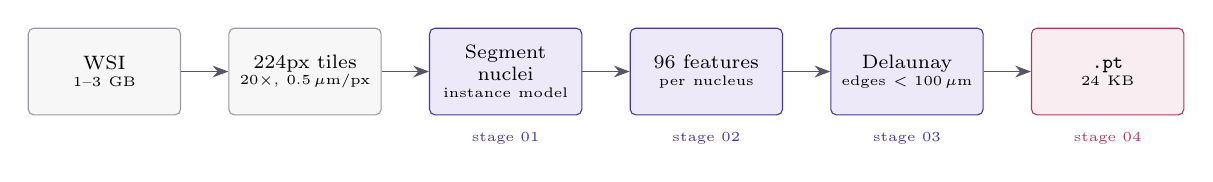
\begin{tikzpicture}[
      node distance=6mm,
      box/.style={draw=inkgrey!60, fill=black!3, rounded corners=2pt,
                  minimum height=11mm, text width=17mm, align=center,
                  font=\scriptsize},
      hbox/.style={box, draw=haem, fill=haemlight},
      ebox/.style={box, draw=eosin, fill=eosinlight},
      ar/.style={-{Stealth[length=2mm]}, draw=inkgrey}
    ]
    \node[box]  (a) {WSI\\[-2pt]\tiny 1--3 GB};
    \node[box, right=of a]  (b) {224px tiles\\[-2pt]\tiny 20$\times$, 0.5\,\um/px};
    \node[hbox, right=of b] (c) {Segment nuclei\\[-2pt]\tiny instance model};
    \node[hbox, right=of c] (d) {96 features\\[-2pt]\tiny per nucleus};
    \node[hbox, right=of d] (e) {Delaunay\\[-2pt]\tiny edges $<100$\,\um};
    \node[ebox, right=of e] (f) {\texttt{.pt}\\[-2pt]\tiny 24 KB};
    \draw[ar] (a)--(b); \draw[ar] (b)--(c); \draw[ar] (c)--(d);
    \draw[ar] (d)--(e); \draw[ar] (e)--(f);
    \node[below=1mm of c, font=\tiny, text=haem] {stage 01};
    \node[below=1mm of d, font=\tiny, text=haem] {stage 02};
    \node[below=1mm of e, font=\tiny, text=haem] {stage 03};
    \node[below=1mm of f, font=\tiny, text=eosin] {stage 04};
  \end{tikzpicture}
  \end{center}

  \vspace{0.2em}
  \begin{itemize}\small
    \item Tissue is separated from background, rescaled to $20\times$
          magnification (0.5\,\um{} per pixel), then cut into non-overlapping
          $224 \times 224$ tiles.
    \item A \hl{nuclei instance segmentation model} detects every individual
          nucleus. The surrounding tissue is discarded, leaving a cell-centric
          representation.
    \item Each nucleus becomes a \hl{node} carrying 96 descriptors.
          \hl{Delaunay triangulation} connects neighbouring cells, and edges
          longer than 100\,\um{} are cut as biologically implausible.
    \item Each edge is weighted by the distance between the two cells, in microns.
  \end{itemize}

\end{frame}

% ------------------------------------------------------------- 6
\begin{frame}[fragile]{Methodology 2: what a \texttt{.pt} file actually contains}

  \texttt{.pt} is simply PyTorch's save format. In GrapHist, each one holds
  \textbf{one cell graph for one tile}:

  \vspace{0.4em}
{\footnotesize
\begin{verbatim}
Data(x=[31, 96], edge_index=[2, 81], edge_attr=[81, 1],
     sample_id='Adrenal_gland_1_01171', labels=[31])      # 16,320 bytes
\end{verbatim}
}

  \vspace{0.2em}
  \begin{center}\footnotesize
  \begin{tabular}{@{}lll@{}}
    \toprule
    \textbf{Field} & \textbf{Shape} & \textbf{Meaning} \\
    \midrule
    \texttt{x}          & [31, 96] & 31 nuclei, each described by 96 numbers \\
    \texttt{edge\_index}& [2, 81]  & 81 connections between nuclei \\
    \texttt{edge\_attr} & [81, 1]  & length of each connection, in microns \\
    \texttt{labels}     & [31]     & the cell type of each nucleus \\
    \bottomrule
  \end{tabular}
  \end{center}

  \vspace{0.5em}
  \begin{alertblock}{The key point: the transformation is one way}
    \textbf{No pixels survive.} A nucleus that was hundreds of pixels of stained
    image is now 96 numbers. One slide becomes about 11,000 \texttt{.pt} files of
    roughly 24 KB each. Because the authors published these finished files, we
    did not have to rebuild them.
  \end{alertblock}

\end{frame}

% ------------------------------------------------------------- 7
\begin{frame}{Methodology 3: the architecture, handling mixed neighbourhoods}

  \begin{block}{The problem a normal graph network has here}
    \footnotesize Standard graph networks \emph{average} each cell with its
    neighbours, which assumes neighbours are similar. In a tumour a cancer cell
    sits beside an immune cell, so averaging destroys the very contrast a
    pathologist looks for.
  \end{block}

  {\small GrapHist uses \hl{Adaptive Channel Mixing (ACM)}. Every layer passes the
  graph through \textbf{three channels at once}:}\vspace{-0.2em}

  \begin{center}\scriptsize
  \begin{tabular}{@{}lll@{}}
    \toprule
    \textbf{Channel} & \textbf{Operator} & \textbf{What it does} \\
    \midrule
    Low-pass  & $A_L = (I + A_{rw})/2$ & blends a cell with its neighbours, smoothing uniform tissue \\
    High-pass & $A_H = (I - A_{rw})/2$ & takes the \emph{difference} from neighbours, sharpening boundaries \\
    Identity  & $A_I = I$              & keeps the cell's own features untouched \\
    \bottomrule
  \end{tabular}
  \end{center}

  \begin{alertblock}{What makes it ``adaptive''}
    \footnotesize For \textbf{each cell separately}, the network scores all three
    channels and takes a \emph{learned} weighted blend. A cell on a tumour
    boundary can lean on the high-pass channel while a cell inside uniform tissue
    leans on the low-pass one. Two extras help: a \hl{virtual node} joined to
    every cell for long-range context, and \hl{jumping knowledge}, which
    combines all layers.
  \end{alertblock}

\end{frame}

% ------------------------------------------------------------- 8
\begin{frame}{Methodology 4: self-supervised pre-training}

  No labels are used at this stage. The model learns by \textbf{hiding parts of
  the graph and reconstructing them}.

  \vspace{0.5em}
  \begin{enumerate}\small
    \item Randomly hide the features of a subset of cells in the graph.
    \item An \hl{encoder} reads the corrupted graph and produces an embedding for
          every cell.
    \item The hidden cells are masked again inside that embedding.
    \item A \hl{decoder} tries to reconstruct their original 96 features.
    \item The model is rewarded for reconstructing them accurately.
  \end{enumerate}

  \vspace{0.6em}
  \begin{block}{Why this works}
    \small To guess a hidden cell's features, the model has no choice but to read
    the cells around it. It therefore learns \emph{cellular context} on its own,
    from 11.1 million graphs, without a single human label.
  \end{block}

  \vspace{0.3em}
  {\footnotesize \textbf{Outcome:} a \hl{9.50M parameter} encoder, pre-trained
  once and released as \texttt{graphist.pt}. This is the checkpoint we evaluate.}

\end{frame}

% ------------------------------------------------------------- 9
\begin{frame}{Methodology 5: how the model is evaluated}

  The encoder is \hl{frozen}. It is never fine-tuned. Only a small classifier on
  top is trained, which tests the \emph{quality of the representation itself}.

  \vspace{0.5em}
  \begin{center}\small
  \begin{tabular}{@{}lll@{}}
    \toprule
    \textbf{Scale} & \textbf{How the embedding is built} & \textbf{Classifier} \\
    \midrule
    Cell   & the cell embedding, used directly & logistic regression \\
    Region & average of all cell embeddings in the region & logistic regression \\
    Slide  & attention pooling over region embeddings & attention MIL \\
    \bottomrule
  \end{tabular}
  \end{center}

  \vspace{0.6em}
  \begin{block}{Why freeze the encoder?}
    \small If the encoder were fine-tuned, a good score could come from the
    fine-tuning rather than from the pre-training. Freezing it means the score
    reflects only what self-supervised pre-training actually learned.
  \end{block}

\end{frame}

% ------------------------------------------------------------- 11
\begin{frame}{Understanding the metrics: what each number means}

  All four are reported as percentages, and higher is better for all four.

  \vspace{0.2em}
  \begin{center}\footnotesize
  \begin{tabular}{@{}p{2.4cm}p{9.8cm}@{}}
    \toprule
    \textbf{Metric} & \textbf{What it measures} \\
    \midrule
    \hl{Macro F1} &
    Balance of precision and recall, computed \emph{separately for each cell
    type} and then averaged with equal weight, so a model that ignores rare cell
    types is heavily punished. This is the headline metric. \\
    \hl{Balanced accuracy} &
    The average, across classes, of ``what fraction of this class did we
    correctly find?''. Random guessing scores $1/k$ for $k$ classes, so 20\% for
    PanNuke's 5 classes. \\
    \hl{AUROC} &
    The probability the model ranks a random positive example above a random
    negative one. 50 is random and 100 is perfect. It measures \emph{ranking
    quality} rather than decisions. \\
    \hl{AUPRC} &
    Area under the precision--recall curve. Unlike AUROC it ignores true
    negatives, making it the more honest metric when a class is rare, which is
    the normal situation in cell typing. \\
    \bottomrule
  \end{tabular}
  \end{center}

  \vspace{0.2em}
  {\scriptsize \textbf{$\Delta$} on the next slide is the absolute gap between
  our value and the paper's, in percentage points. Smaller is better.}

\end{frame}

% ------------------------------------------------------------- 12
\begin{frame}{Results: cell level, ours vs the paper}

  {\scriptsize Reproduced using \textbf{only what the authors released}: the
  pre-trained checkpoint, the published datasets and the public code.}
  \begin{center}\scriptsize
  \begin{tabular}{@{}llrrr@{}}
    \toprule
    \textbf{Setting} & \textbf{Metric} & \textbf{Ours} & \textbf{Paper} & \textbf{$\Delta$} \\
    \midrule
    PanNuke PanCancer & Macro F1      & 59.54 $\pm$ 0.08 & 59.47 $\pm$ 0.11 & 0.07 \\
                      & Balanced acc  & 68.70 $\pm$ 0.98 & 68.73 $\pm$ 0.96 & 0.03 \\
                      & AUROC         & 89.68 $\pm$ 0.04 & 89.57 $\pm$ 0.05 & 0.11 \\
                      & AUPRC         & 66.45 $\pm$ 0.85 & 66.30 $\pm$ 0.94 & 0.15 \\
    PanNuke Breast    & Macro F1      & 56.39 $\pm$ 0.06 & 56.43 $\pm$ 0.04 & 0.04 \\
                      & Balanced acc  & 57.49 $\pm$ 0.07 & 57.49 $\pm$ 0.07 & \textcolor{goodgreen}{\textbf{0.00}} \\
                      & AUROC         & 85.49 $\pm$ 8.13 & 85.30 $\pm$ 8.07 & 0.19 \\
                      & AUPRC         & 61.94 $\pm$ 0.27 & 61.85 $\pm$ 0.30 & 0.09 \\
    NuCLS main        & Macro F1      & 25.96 $\pm$ 2.51 & 26.57 $\pm$ 2.16 & 0.61 \\
                      & AUROC         & 72.41 $\pm$ 1.68 & 71.49 $\pm$ 1.55 & 0.92 \\
    NuCLS super       & Macro F1      & 46.52 $\pm$ 2.53 & 46.24 $\pm$ 3.89 & 0.28 \\
                      & Balanced acc  & 50.96 $\pm$ 5.28 & 48.04 $\pm$ 3.14 & 2.92 \\
    \bottomrule
  \end{tabular}
  \end{center}

  {\scriptsize
  \hl{PanNuke reproduces:} eight metrics, largest deviation 0.19 points, one exact
  match. The odd $\pm 8.07$ spread on Breast AUROC looks like a typo, but it
  reproduces as $\pm 8.13$ (one weak fold: 73.99 against 91.56 and 90.91).
  \textbf{Reproducing an anomaly of that shape is stronger evidence than a clean
  average.}}

\end{frame}

% ------------------------------------------------------------- 13
\begin{frame}{Results: region level and structural checks}

  \begin{columns}[T]
    \begin{column}{0.52\textwidth}
      \textbf{Region level}
      \begin{center}\footnotesize
      \begin{tabular}{@{}lrrr@{}}
        \toprule
        \textbf{Dataset} & \textbf{Ours} & \textbf{Paper} & \textbf{$\Delta$} \\
        \midrule
        BreakHis & 90.43 & 89.37 & $+1.06$ \\
        BRACS    & 62.26 & 60.30 & $+1.96$ \\
        \bottomrule
      \end{tabular}
      \end{center}
      {\scriptsize Macro F1. Both land \emph{within two points} of the paper's
      pipeline while using one graph for the whole region instead of splitting it
      into tiles. This supports the paper's claim that performance stays stable
      across patch sizes.}
    \end{column}
    \begin{column}{0.46\textwidth}
      \textbf{Structural checks, all verified}
      \begin{itemize}\footnotesize
        \item Parameter counts: exact at all three model sizes
        \item 96 node features: confirmed by tracing the extraction code
        \item Graph statistics: match to two decimals
        \item Class distributions: all 16 counts exact
      \end{itemize}
    \end{column}
  \end{columns}

  \vspace{0.5em}
  \begin{block}{What this establishes}
    \small The published model behaves exactly as reported. That matters for the
    next part: it gives us a \emph{trustworthy baseline} to measure any proposed
    change against.
  \end{block}

\end{frame}

% ------------------------------------------------------------- 14
\begin{frame}{Research gap: the virtual node is applied in the wrong space}

  Recall the \hl{virtual node}, the extra node joined to every cell to carry
  long-range context. Its connection strength has to be set to some value.

  \vspace{0.4em}
  \begin{columns}[T]
    \begin{column}{0.48\textwidth}
      \begin{block}{What the paper says}
        \small Its edge weights are set to \emph{``the mean of all edge weights in
        the pre-training dataset''}.
      \end{block}
    \end{column}
    \begin{column}{0.48\textwidth}
      \begin{alertblock}{What the code does}
        \small Uses a fixed value of \texttt{22.5}, and inserts it \emph{after}
        all the other edge weights have already been rescaled.
      \end{alertblock}
    \end{column}
  \end{columns}

  \vspace{0.5em}
  After rescaling, the average edge weight is 18.627 with a spread of 12.735, so
  the correct value on that scale is $(22.5 - 18.627)/12.735 = \mathbf{0.304}$.

  \vspace{0.4em}
  \begin{center}
  \fbox{\parbox{0.88\textwidth}{\centering
  The inserted value is \al{roughly 74 times too large.}\\
  Converted back, 22.5 corresponds to about 305\,\um, which is three times the
  100\,\um{} biological cutoff the graphs themselves enforce.}}
  \end{center}

\end{frame}

% ------------------------------------------------------------- 15
\begin{frame}{Research gap: what we measured}

  Measured on 300 real PanNuke graphs.

  \vspace{0.3em}
  \begin{center}\footnotesize
  \begin{tabular}{@{}lrrr@{}}
    \toprule
    \textbf{Configuration} & \textbf{bad degrees} & \textbf{neighbour vs self} & \textbf{low vs high similarity} \\
    \midrule
    As shipped, value 22.5          & 0.0\%  & 0.080 & \al{0.992} \\
    Simple fix, value 0.304         & \al{57.8\%} & 1.009 & $-0.012$ \\
    Distance kernel (our proposal)  & \textcolor{goodgreen}{0.0\%} & 0.787 & \textcolor{goodgreen}{0.320} \\
    \bottomrule
  \end{tabular}
  \end{center}

  \vspace{0.3em}
  \begin{alertblock}{Finding A: the headline mechanism is inert}
    \footnotesize The virtual node absorbs \textbf{99.92\%} of everything each
    cell aggregates. As a result the low-pass and high-pass channels come out
    \textbf{99.2\% identical}. \emph{The adaptive channel mixing has nothing left
    to mix}, so the mechanism the paper's argument rests on is not actually
    operating.
  \end{alertblock}

  \begin{block}{Finding B: the real issue is where the value is applied}
    \footnotesize Rescaled weights can be \emph{negative}, but the averaging step
    requires positive ones: \textbf{56\% of cells have a negative total}. The
    22.5 value was accidentally hiding this, so simply correcting it to 0.304
    makes things \emph{worse}. A positive distance-based weighting fixes both
    problems at once.
  \end{block}

\end{frame}

% ------------------------------------------------------------- 16
\begin{frame}{Future work: testing the correction}

  \begin{block}{Honest positioning}
    \footnotesize The authors' own dataset notes call distance-based weights
    ``counterintuitive'' and suggest trying the inverse of distance, so
    \textbf{the idea of a different weighting is not ours}. But they never
    measured it, every published number uses the original weighting, and their
    notes say nothing about the virtual node, the 99.92\% share, or the negative
    totals. \emph{That interaction is our contribution.}
  \end{block}

  {\small\textbf{Proposed experiment:} three full pre-training runs on identical
  data, epochs and seed, changing only the edge weighting.}

  \begin{center}\scriptsize
  \begin{tabular}{@{}llll@{}}
    \toprule
    \textbf{Arm} & \textbf{Edge weight} & \textbf{Virtual node} & \textbf{Purpose} \\
    \midrule
    A & rescaled distance (as shipped) & 22.5 & reproduce the checkpoint, validate our pipeline \\
    B & inverse of distance & matched mean & test the authors' own unmeasured suggestion \\
    C & distance kernel, corrected & matched mean & our proposed correction \\
    \bottomrule
  \end{tabular}
  \end{center}

  {\scriptsize
  \textbf{Feasible:} the full 11.1 million graph pre-training corpus \emph{is}
  published, with official splits, and an A100 is available at roughly two days
  per arm.
  \textbf{Prediction:} the correction should help most where mixed neighbourhoods
  matter, that is, boundary cell types in NuCLS and PanNuke, measured against the
  baseline our reproduction established.}

\end{frame}

% ------------------------------------------------------------- 17
\begin{frame}{Conclusion}

  \begin{block}{The published results hold}
    \small All eight PanNuke metrics reproduce within 0.19 percentage points, the
    region-level results within two points, and every structural claim checks out
    exactly. \textbf{GrapHist's reported performance is real.}
  \end{block}

  \vspace{0.3em}
  \begin{alertblock}{But the mechanism behind it is not the one described}
    \small The virtual node absorbs \textbf{99.92\%} of everything each cell
    aggregates, leaving the low-pass and high-pass channels \textbf{99.2\%
    identical}. The adaptive channel mixing that the paper's whole argument rests
    on is not actually operating.
  \end{alertblock}

  \vspace{0.3em}
  \begin{block}{The cause is precise and the fix is testable}
    \small The value is applied on the wrong scale, and correcting it naively
    makes things worse. A positive distance-based weighting repairs both the
    scale and the negative-total problem at once.
  \end{block}

  \vspace{0.4em}
  {\small \textbf{Next step:} three controlled pre-training runs on the published
  corpus, to measure what the correction is actually worth.}

\end{frame}

% ------------------------------------------------- backup (not counted)
\appendix

\begin{frame}[noframenumbering]{Backup: why do our numbers differ from the paper's?}

  \begin{alertblock}{First, the premise}
    \footnotesize \textbf{We did not retrain anything.} The encoder is the
    authors' released checkpoint, frozen. There is no random initialisation and
    no seed in our pipeline, so training randomness cannot explain any of this.
  \end{alertblock}

  \vspace{0.2em}
  \begin{center}\scriptsize
  \begin{tabular}{@{}lll@{}}
    \toprule
    \textbf{Result family} & \textbf{$\Delta$} & \textbf{Actual cause} \\
    \midrule
    PanNuke      & 0.00 to 0.19 & floating-point noise: A100 GPU vs Apple CPU, and newer libraries \\
    NuCLS        & 0.28 to 3.05 & the official fold splits were never published, so we rebuilt them \\
    Region level & $+1.06$, $+1.96$ & different input: one whole-region graph instead of patches \\
    \bottomrule
  \end{tabular}
  \end{center}

  \vspace{0.2em}
  {\scriptsize
  \hl{PanNuke.} Float32 sums accumulate in a different \emph{order} on a GPU than
  on a CPU. Those 1e-6 differences pass through 5 layers and then hit a linear
  decision boundary, so a few cells out of 163,163 flip class.
  \textbf{This is the floor for cross-platform reproduction.}

  \vspace{0.3em}
  \hl{NuCLS.} A different fold assignment is a different experiment, so the
  numbers \emph{should} move. The defence is that our gaps are smaller than the
  paper's own fold-to-fold spread: Macro F1 $0.28$ vs $\pm 3.89$, balanced
  accuracy $2.92$ vs $\pm 3.14$, AUROC $1.16$ vs $\pm 2.08$, AUPRC $3.05$ vs
  $\pm 2.59$.

  \vspace{0.3em}
  \hl{Evidence it is noise, not error.} The odd $\pm 8.07$ spread on Breast AUROC
  is caused by one weak fold (73.99 against 91.56 and 90.91). We reproduced it as
  $\pm 8.13$. \textbf{A real methodological difference would smear that artefact
  out, not reproduce its exact shape.}}

\end{frame}

\end{document}
